%! TeX root = master.tex
% !TEX program = lualatex

\lecture{1}{2026-09-09}{Introduction and the Secretary Problem}{}

\section{Introduction to Online Decision-Making}

\subsection{What is online (sequential) decision-making?}

Online, or sequential, decision-making refers to settings in which an \emph{agent} repeatedly decides on an action, receives feedback from the environment, and then decides on another action, and so on. Usually, the sequence of decisions coincides with time.

Three ingredients characterize this class of problems:
\begin{itemize}
    \item \textbf{Sequential}: the agent takes a decision, observes feedback, takes another decision, etc.
    \item \textbf{Decision}: a decision is \emph{irrevocable} -- once taken, it cannot be undone.
    \item \textbf{Uncertainty}: the environment is not known in advance, so the agent must \emph{probe} it; the future is not known either, so the agent must rely on statistical assumptions.
\end{itemize}

\begin{example}[Teaching a new class]
Consider a class being taught for the first time. The instructor has some prior information (student background, curriculum, goals) and a finite horizon (e.g., 14 weeks of lectures). Uncertainties include the students' background, how content is best acquired, and extraneous effects (other courses, external events). Every lecture reveals new information (questions asked, homework performance, midterm results), based on which the instructor takes actions: tweaking the lectures, and students may drop or join the class.
\end{example}

\subsection{Three classes of models}

This course studies three families of sequential decision problems, in increasing order of complexity.

\begin{itemize}
    \item \textbf{Optimal stopping} (the secretary problem, covered this week): the horizon is finite and the agent must commit to a choice.
    \item \textbf{Bandits} (about 6 weeks): the agent repeatedly decides which \emph{arm} (option) to play; outcomes are random, and there is an optimal arm that is not known a priori. The agent must learn the value of the different options over time.
    \item \textbf{Reinforcement learning} (about 6 weeks): the agent learns to interact with an environment that has a \emph{state} (i.e., memory); outcomes of actions are random and rewards can be delayed.
\end{itemize}

\subsubsection*{Example: optimal stopping -- finding a parking spot}

Consider the problem of finding a parking spot close to a destination, with limited lookahead: if the destination is reached without having found a spot, this is a failure. If a spot is found, the reward equals minus the distance walked to the destination. There is a clear tradeoff: parking too early means a lot of walking, while parking too late risks missing the destination entirely (or arriving too late). How should one park optimally?

\subsubsection*{Example: multi-armed bandits}

In a multi-armed bandit problem, the set of actions is called the set of \emph{arms}. The agent takes a sequence of decisions on which action (arm) to pull, and receives a reward after each action according to some reward function. In a \emph{stochastic} bandit, the reward is random, and is independent of everything except the choice of action taken. The name traces back to Thompson [1933].

\begin{example}[Clinical trial]
Consider running a clinical trial without unnecessarily harming patients. The gold standard for clinical trials is to randomize: randomly give each patient the drug or a placebo. There is always a nonzero probability that the medicine does not work, or is even more harmful than the placebo -- so when should we decide that this is unlikely enough that we should stop giving placebos?

The classical statistical approach fixes a confidence criterion (a $p$-value) beforehand, which determines the size $n$ of the trial (how many patients are needed): more patients give higher confidence. But if the medicine works very well (or seems worse than the placebo), many people stay sick needlessly while the trial runs to completion. Ideally, we should be able to abort the trial early once the outcome becomes clear -- but what if this apparent trend was only a fluke?

The question is therefore: instead of assigning treatments purely at random, how do we decide, for each new patient arriving sequentially, whether to give the drug or the placebo, using all information available so far?
\end{example}

\begin{remark}[The importance of the horizon]
Suppose every arm $a$ generates a reward distributed like $X_a$, independent of everything else. How would you play if $n = 1$? How would you play if $n \to \infty$? This is analogous to portfolio choice: stocks have higher expected return but also higher volatility, while bonds have lower return and lower volatility -- investment advice differs for a 20-year-old versus a 50-year-old. The horizon over which the agent needs to perform well is a key parameter of the problem.
\end{remark}

\subsubsection*{Example: reinforcement learning -- Atari Pong}

Consider learning to play a computer game (e.g., Atari Pong). We do not (or cannot) program the rules of the game and then compute the optimal move analytically. Instead, an algorithm should observe and master the game as quickly as possible by playing and observing. Feedback comes as reward signals ($+1$ if the agent scores, $-1$ if the adversary scores). The environment has a \emph{state} (e.g., ball position and velocity, own position), and the right action depends on this state. A key additional difficulty is that signals arrive \emph{with delay}.

\subsection{Probability tools we will need}

\subsubsection*{Concentration results}

Concentration results describe the limiting behavior of probability distributions at different ``zoom levels''. Suppose $X_1, \dots, X_n$ is a sequence of i.i.d.\ random variables, and let $S_n = \sum_{i=1}^n X_i$.

\begin{itemize}
    \item \textbf{Law of Large Numbers}: $\dfrac{S_n}{n} \to \mu$ (the average converges to the mean). This is an \emph{asymptotic} statement ($n \to \infty$) and gives no information for a specific finite $n$.
    \item \textbf{Central Limit Theorem}: $\dfrac{S_n - n\mu}{\sqrt{n}} \to \mathcal{N}(0, \sigma^2)$, characterizing the ``typical'' (standard) deviation from the mean.
    \item \textbf{Chernoff bound}: $\mathbb{P}\left(\dfrac{S_n}{n} \geq \mu + \epsilon\right) \leq \exp(-f(\epsilon) n)$, giving a more precise tail behavior for a specific finite $n$, i.e., the probability of very large departures from the mean.
\end{itemize}

\subsubsection*{Markov chains}

We are familiar with sequences of i.i.d.\ random variables $X_1, \dots, X_n$ (LLN, CLT, etc.). To add ``a bit of dependence'', consider $(X_1, X_2, X_3)$ with $X_1 \perp X_3 \mid X_2$: this defines a \emph{Markov chain}. Now let the number of variables go to infinity, assume homogeneity (the probabilistic relationship between neighboring variables is the same everywhere) and discrete random variables. The chain is then described by a transition matrix $P$, with $P_{ij} = \mathbb{P}(X_n = j \mid X_{n-1} = i)$.

Depending on $P$, sets of states can have different long-term behaviors (absorbing, transient, periodic). Under certain conditions on $P$, the long-term behavior of the chain converges (\emph{ergodicity}); in this ergodic regime, one is interested in the \emph{stationary distribution} $\pi$, the normalized solution of the eigenvector problem $\pi = \pi P$.

\subsubsection*{Markov Decision Processes (MDPs)}

An MDP formalizes decision-making in an environment with state. A \emph{policy} \textcolor{red}{$\pi$} maps a \textcolor{blue}{state} to an \textcolor{green}{action}. The goal is to maximize the reward over a long time horizon.
\begin{center}
   
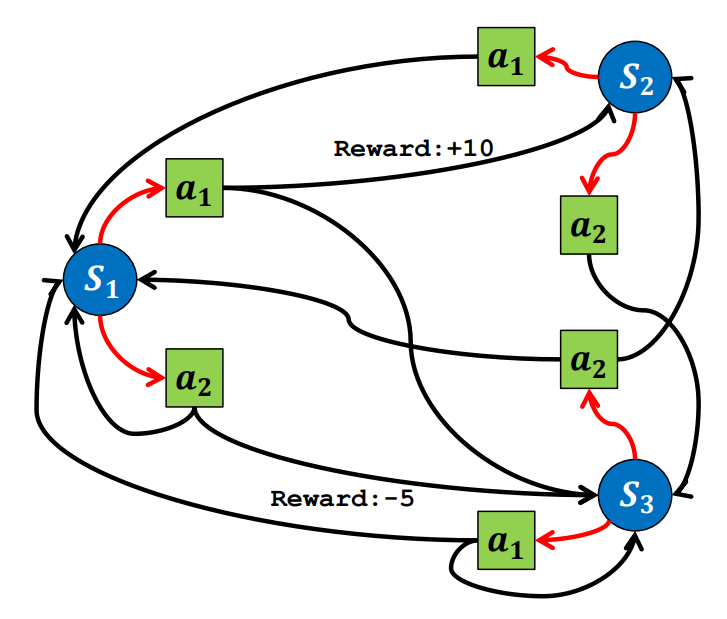
\includegraphics[width=0.4\linewidth]{images/img_20260919_204416.png}
\end{center}

\begin{example}[Learning to walk]
Model: physics of limbs, gravitation, friction with the ground. Actions: move joints. Rewards: getting to some place. Key challenges: large, continuous state and action spaces. This topic will not be covered in detail in this course.

\end{example}

\subsection{Reinforcement learning vs.\ supervised learning}

In classical supervised learning: labeled data is collected, a model is trained to give good predictions, and at test time the model is deployed and used.

In the real world, data keeps accruing during test/deployment time, which can be used to refine the model; moreover, the system might not be stationary, requiring adaptation (e.g., periodic retraining). Updating the model may also influence the future data distribution: e.g., in a recommender system, people consume the items the system recommends, so future data becomes biased toward recommended items -- a potential positive feedback loop.

Reinforcement learning integrates ``training'' (\emph{explore}) with ``testing'', i.e., using the model to accomplish something (\emph{exploit}).

\subsection{Key concept: the explore-exploit tradeoff}

\begin{definition}[Explore-exploit tradeoff]
\textbf{Explore}: collect samples to learn about the environment/model -- somewhat like the training set in supervised learning; the agent does not attempt to take good decisions, but to understand the problem.

\textbf{Exploit}: try to take good actions/decisions -- somewhat like the test set in supervised learning; the agent does try to take good decisions, even though the model is still noisy.
\end{definition}

This tradeoff recurs across all the examples seen so far:
\begin{itemize}
    \item \textbf{Parking}: explore (look for a better spot) vs.\ exploit (park now).
    \item \textbf{Clinical trial}: explore (give a random treatment) vs.\ exploit (give the treatment believed best).
    \item \textbf{Pong}: explore (random move) vs.\ exploit (best-guess move).
\end{itemize}

This course develops probabilistic models for such situations, algorithms to handle them, and analysis of the optimality of these algorithms.

\subsection{Prerequisites}

This is essentially a probability class; introductory probability is enough, although mathematical maturity helps. It is not a bad idea to take \emph{Modèles stochastiques} in parallel, since there is some overlap (mostly Markov chains) -- however, this course (PODM) is self-contained. Solid prerequisites in basic probability are required.

\section{Optimal Stopping: the Secretary Problem}

\subsection{Problem statement}

\begin{definition}[Secretary problem, a.k.a.\ ``apartment hunting problem'']
You are looking for an apartment to rent on a hot market: you must take it or leave it forever, on the spot. You know the number of options in advance: $n$ apartments will be viewed, and you need shelter after the last one. Every apartment has a quality level $x_i$, drawn i.i.d.\ from some \emph{unknown} law -- equivalently, one may simply assume that the apartments are viewed in a uniformly random order, with no information about the underlying probability law. The only information available at step $i$ is the values $x_1, \dots, x_i$ seen so far (or, more precisely, their relative ranking).

Decisions are irrevocable: sign the lease immediately, or that apartment is gone forever. The goal is to maximize the probability of selecting the overall best apartment among the $n$.
\end{definition}

This model captures many practical situations with the same flavor, e.g.:
\begin{itemize}
    \item Resource allocation: how much effort to spend searching and evaluating before hiring a candidate or selecting a vendor.
    \item Online auctions: updating one's own bid upon observing other bids.
    \item Acquiring friendships/social contacts over a lifetime.
\end{itemize}
The problem is also known under other names: the \emph{marriage problem}, the \emph{sultan's dowry}, or the \emph{googol game}.

\subsection{Optimal policy: threshold structure}

\begin{theorem}[Form of the optimal policy]
The optimal policy is necessarily of the following form, for some constant threshold $k$:
\begin{enumerate}
    \item[(1)] If $x_i$ is \emph{not} a new maximum (relative to $x_1, \dots, x_{i-1}$), continue.
    \item[(2)] If $x_i$ \emph{is} a new maximum, stop (commit) if $i \geq k$; otherwise continue.
\end{enumerate}
\end{theorem}

\begin{proof}[Justification]
\textbf{Why (1)?} Stopping on a value that is not a new maximum is guaranteed to fail (the true best has already appeared, or will appear later and we have already committed to a non-optimal value) -- this is never a good idea.

\textbf{Why (2)?} We claim the optimal policy continues before $k$ and stops at or after $k$ upon seeing a new maximum, i.e., the policy is \emph{monotonic}: if we decide to stop upon seeing a new maximum-so-far at position $i$, we must also decide to stop upon seeing a new maximum-so-far at any $j > i$.

To see this, condition on observing the maximum over $x_1, \dots, x_i$ seen so far (i.e., $x_i > \max(x_1, \dots, x_{i-1})$). The probability of success if we commit to $x_i$ is exactly $i/n$: the overall maximum is uniformly distributed over $\{1, \dots, n\}$, so this conditional probability of success is \emph{increasing} in $i$. On the other hand, the (unconditional) probability of seeing a new maximum-so-far at step $i$ is \emph{decreasing} in $i$. Hence, if the tradeoff (value of stopping vs. probability of the opportunity arising) is favorable at $i$, it is even more favorable at any $j > i$.
\end{proof}

\subsubsection*{Small cases: $n = 1, 2, 3$}

\begin{itemize}
    \item $n=1$: nothing to do, commit to the only option.
    \item $n=2$: the best is first with probability $1/2$ and second with probability $1/2$. Either commit to the first, or (implicitly) commit to the second (=last) if not; $\mathbb{P}(\text{success}) = 1/2$.
    \item $n=3$: the smallest $n$ for which we actually ``make a decision''. With $k=2$, we use the comparison between the first and second position to decide whether to take the second or the third apartment.
\end{itemize}

The table below enumerates all $3! = 6$ orderings of the ranks $\{1,2,3\}$ (1 = best) and the resulting success probability for each candidate threshold $k \in \{1,2,3\}$.

\begin{center}
\begin{tabular}{c|c|c|c}
 & $k=1$ & $k=2$ & $k=3$ \\
\hline
 &$\textcolor{red}{1}\,2\,3$ & $1\,\textcolor{red}{2}\,3$ & $1\,2\,\textcolor{green}{3}$ & \\ 
 &$\textcolor{red}{1}\,3\,2$ & $1\,\textcolor{green}{3}\,2$ & $1\,3\,\textcolor{red}{2}$ & \\ 
 &$\textcolor{red}{2}\,1\,3$ & $2\,1\,\textcolor{green}{3}$ & $2\,1\,\textcolor{green}{3}$ & \\
 &$\textcolor{red}{2}\,3\,1$ & $2\,\textcolor{green}{3}\,1$ & $2\,3\,\textcolor{red}{1}$ & \\
 &$\textcolor{green}{3}\,1\,2$ & $3\,1\,\textcolor{red}{2}$ & $3\,1\,\textcolor{red}{2}$ & \\
 &$\textcolor{green}{3}\,2\,1$ & $3\,2\,\textcolor{red}{1}$ & $3\,2\,\textcolor{red}{1}$ & \\
\hline
$\mathbb{P}(\text{success})$ & $1/3$ & $1/2$ & $1/3$
\end{tabular}
\end{center}

The threshold $k=2$ is optimal for $n=3$, giving $\mathbb{P}(\text{success}) = 1/2$.

\subsection{General optimal threshold $k$}

Let $U$ denote the index (position) of the true overall maximum; note that $U \sim \mathrm{Unif}\{1, \dots, n\}$. Let $Z$ denote the output of the policy (its guess for $U$), and let $E$ be the event ``success'', i.e., the policy chooses index $i$ and $i$ is indeed the best. Then:
\[
\mathbb{P}(E) = \sum_{i=k}^{n} \mathbb{P}(Z = i \cap U = i) = \sum_{i=k}^{n} \mathbb{P}(Z = i \mid U = i)\, \mathbb{P}(U = i), \qquad \mathbb{P}(U=i) = \frac{1}{n}.
\]

\textbf{Computing $\mathbb{P}(Z = i \mid U = i)$.} The event $\{Z = i \mid U = i\}$ holds when $i$ is the overall best (so rule (2) is triggered with certainty at step $i$: success), \emph{provided} the policy has not stopped earlier. This requires that all previous best-so-far values occur \emph{before} $k$. Conditional on $\{U = i\}$, where is the best value among $x_1, \dots, x_{i-1}$ (not necessarily the second-best overall, which could occur after $i$ -- just the best \emph{so far})? All we know is that it is not at $i$, so its position is uniformly distributed over $\{1, \dots, i-1\}$. Hence:
\[
\mathbb{P}(Z = i \mid U = i) = \mathbb{P}\big(\mathrm{Unif}(i-1) \in \{k-1\}\big)\cdot(k-1) = \frac{k-1}{i-1}.
\]

\begin{center} 
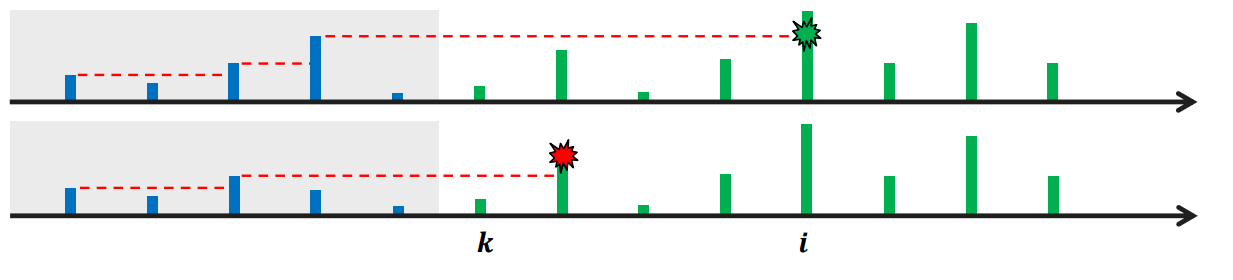
\includegraphics[width=\linewidth]{images/img_20260919_211642.png}
\end{center}


\subsubsection*{Finite $n$}

Combining the two pieces:
\[
\mathbb{P}(E) = \sum_{i=k}^{n} \frac{k-1}{i-1} \cdot \frac{1}{n} = \frac{k-1}{n} \sum_{i=k}^{n} \frac{1}{i-1} = \frac{1}{n}\big(H_{n-1} - H_{k-2}\big),
\]
where $H_m = \sum_{j=1}^m \frac{1}{j}$ is the $m$-th harmonic number. Optimizing over $k$ for each $n$ gives:

\begin{center}
\begin{tabular}{c|cccccccccccccccc}
$n$ & 1 & 2 & 3 & 4 & 5 & 6 & 7 & 8 & 9 & 10 & 20 & 30 & 40 & 50 & 100 & 1000 \\
\hline
$k$ & 1 & 1 & 2 & 2 & 3 & 3 & 3 & 4 & 4 & 4 & 7 & 11 & 15 & 18 & 37 & 369 \\
\hline
$\mathbb{P}(E)$ & 1 & 0.5 & 0.5 & 0.458 & 0.433 & 0.428 & 0.414 & 0.410 & 0.406 & 0.399 & 0.384 & 0.379 & 0.376 & 0.374 & 0.371 & 0.368
\end{tabular}
\end{center}

Remarkably, $\mathbb{P}(E)$ appears to converge to a positive constant as $n \to \infty$. Also note that neither $k$ nor $\mathbb{P}(E)$ depends on the distribution of the $x_i$ -- only on $n$.

\subsubsection*{Large $n$: the $1/e$ rule}

Set $x = k/n$. As $n \to \infty$, the sum becomes an integral:
\[
\mathbb{P}(E) \xrightarrow{n \to \infty} x \int_{y=x}^{1} \frac{1}{y}\, dy = -x \ln x.
\]
Optimizing over $x$: setting $\dfrac{d\,\mathbb{P}(E)}{dx} = 0$ gives $x = e^{-1} \approx 37\%$.

\begin{theorem}[The $1/e$ rule]
As $n \to \infty$, the optimal threshold is $k \approx n/e$, and the optimal success probability converges to $1/e \approx 0.368$. Informally: ``look at the first $37\%$ of the candidates without committing, then leap at the next candidate that beats everything seen so far.''
\end{theorem}

\subsection{Random order vs.\ i.i.d.\ random variables}

An important assumption underlying the whole analysis is that we have \emph{no information about future values}. Two ways to phrase this assumption, and why both matter:

\begin{itemize}
    \item \textbf{I.i.d.\ random variables}: the player does not know the underlying distribution. \emph{Counterexample if this fails}: if we knew the distribution of the $x_i$, we could directly compute the probability that $x_i$ is the overall maximum; if this probability is already large, there would be no need to wait until $k$.
    \item \textbf{Rank order}: only the partial order (ranking) of the items seen so far (up to $i$) is available. \emph{Counterexample if this fails}: if $x_i$ revealed its total rank among all $n$ items, we could simply wait for an item ranked \#1 at any time and stop immediately.
\end{itemize}

The need to ``pay'' with some samples in order to discover the distribution and correctly judge future samples is what makes the problem interesting, and is baked into these assumptions.

\subsection{Does the goal matter? Success probability vs.\ expected value}

The optimal policy derived above is specific to the particular criterion adopted, namely maximizing $\mathbb{P}(Z = U)$: it never accepts anything below the maximum-so-far.

Suppose instead we wanted to maximize the \emph{expected value} of the chosen apartment, $\mathbb{E}[x_Z]$ (i.e., rent a \emph{good} apartment, without it being catastrophic if it is not the very best). Does the optimal policy change?

\begin{remark}
Yes, it does. \emph{Counterexample}: suppose we are close to $n$ and we observe the second-best value seen so far -- it is very unlikely that this can still be beaten, so we should take it. In fact, under this new goal, we should accept anything above the \emph{median} of the values seen so far near the end of the sequence. This policy guarantees eventual failure under the previous (probability-of-best) criterion, but performs much better in terms of expected score.
\end{remark}

This illustrates a general lesson: the goal (objective function) fundamentally shapes what the optimal policy looks like.

\subsection{Explore-exploit tradeoff, revisited}

The explore-exploit tradeoff introduced earlier is the key underlying concept of this course:
\begin{itemize}
    \item \textbf{Explore}: make potentially bad decisions (with respect to some specified goal) in order to estimate parameters of the system, helping make better decisions in the future.
    \item \textbf{Exploit}: based on these estimates, make good decisions with respect to the specified goal.
\end{itemize}

In the secretary problem, explore and exploit are \emph{sharply separated}: there are two phases, with an a-priori threshold ($k$) at which the policy switches from one to the other. In bandit problems and in reinforcement learning, exploration and exploitation will instead meld together more gradually:
\begin{itemize}
    \item \textbf{Bandits}: gradually improve estimates of the rewards of different arms, stop playing some arms earlier than others, and gradually optimize the rewards obtained.
    \item \textbf{Reinforcement learning}: gradually exclude states and actions that are unlikely or costly to lead to rewards, driving the system towards good states.
\end{itemize}
 \newpage
